\documentclass[twocolumn]{bmcart}
%\documentclass[smallcondensed]{svjour3}
\usepackage{amsmath,amssymb}

% Use adjustwidth environment to exceed column width (see example table in text)
\usepackage{changepage}
\usepackage[utf8x]{inputenc}
\usepackage[T1]{fontenc}
\usepackage{textcomp,marvosym}

\usepackage{cite}

% Use nameref to cite supporting information files (see Supporting Information section for more info)
\usepackage{nameref}

% line numbers
%\usepackage[right]{lineno}

\usepackage{marginnote}\reversemarginpar

% ligatures disabled
\usepackage{microtype}
\DisableLigatures[f]{encoding = *, family = * }
%\usepackage[table]{xcolor}
\usepackage{tabularx}
\usepackage{array}
\usepackage{multirow}

%\usepackage[aboveskip=1pt,labelfont=bf,labelsep=period,justification=raggedright,singlelinecheck=off]{caption}
\usepackage{caption}
\renewcommand{\figurename}{Fig}

\usepackage{color}

\date{}

%%% Put your definitions there:
\startlocaldefs
\endlocaldefs

\usepackage{gra phicx}

\DeclareMathOperator*{\argmin}{arg\,min}

\usepackage{hyperref}

\begin{document}
%\vspace*{0.2in}

\begin{frontmatter}

\begin{fmbox}
\dochead{Research}

\title{Heart Rate Variability and accelerometry as classification tools for monitoring perceived stress levels: a pilot study on firefighters}

\author[
   addressref={aff1},                   % id's of addresses, e.g. {aff1,aff2}
   corref={aff1},                       % id of corresponding address, if any
   %noteref={n1},                        % id's of article notes, if any
   email={michal.meina@gmail.com}   % email address
]{\inits{MM}\fnm{Michał} \snm{Meina}}
\author[
   addressref={aff2},
   email={sadowska.maria88@gmail.com}
]{\inits{MS}\fnm{Maria} \snm{Sadowska}}
\author[
   addressref={aff1},
   email={trufliczka@gmail.com}
]{\inits{ER}\fnm{Ewa} \snm{Ratajczak}}
\author[
   addressref={aff3},
   email={mozgun@mat.umk.pl}
]{\inits{KR}\fnm{Krzysztof} \snm{Rykaczewski}}
\author[
   addressref={aff2},
   email={joanna.dreszer@gmail.com}
]{\inits{KR}\fnm{Joanna} \snm{Dreszer}}
\author[
   addressref={aff4},
   email={adam.p.krasuski@gmail.com}
]{\inits{KR}\fnm{Adam} \snm{Krasuski}}
\author[
   addressref={aff2},
   email={bibianna.balaj@gmail.com}
]{\inits{KR}\fnm{Bibianna} \snm{Bałaj}}


\address[id=aff1]{%                           % unique id
  \orgname{Department of Physics, Astronomy and Applied Informatics, Nicolaus Copernicus University}, % university, etc
  \street{Grudzi\k{a}dzka 5},                     %
  \postcode{87-100},                                % post or zip code
  \city{Toruń},                              % city
  \cny{Poland}                                    % country
}

\address[id=aff2]{%
  \orgname{Department of Psychology, Faculty of Humanities, Nicolaus Copernicus University},
  \street{Fosa Staromiejska 1a},
  \postcode{87-100},
  \city{Toruń},
  \cny{Poland}
}

\address[id=aff3]{%
  \orgname{The Interdisciplinary Center for Modern Technologies},
  \street{Wileńska 4},
  \postcode{87-100},
  \city{Toruń},
  \cny{Poland}
}

\address[id=aff4]{%
  \orgname{The Main School of Fire Service},
  \street{Słowackiego 52/54},
  \postcode{01-629},
  \city{Warsaw},
  \cny{Poland}
}

\begin{artnotes}
%\note{Sample of title note}     % note to the article
\note[id=n1]{Equal contributor} % note, connected to author
\end{artnotes}

%\end{fmbox}% comment this for two column layout

\begin{abstractbox}

\begin{abstract} % abstract
\textbf{Background} Chronic stress is the main cause of health problem in high risk jobs. Wearable sensors can become ecologically valid method for assessing stress levels in real-life applications. We sought to determine the non-invasive technique for objective stress monitoring.\\
\textbf{Methods} Data were collected during 24-hour shifts, using sensor belts equipped with a dry-lead electrocardiograph (ECG) and a three-axial accelerometer. Evaluation of the stress occurring during fire incidents was gathered by means of a brief self-assessment questionnaire. R-R time series was segmented according to type of physical activity indicated by acceleroemter readings. Those segments were classified for stress/no-stress conditions.\\
\textbf{Results} ROC analysis showed true positive classification for 15\% of incidents (while maintaining almost zero False Positive Rate), which parallels the amount of truly stressful incidents reported in the questionnaires.\\
\textbf{Conclusions} These results show a firm correspondence between the perceived stress level and physiological data. Psychophysiological measurements are reliable indicators of stress even in ecological settings, and appear promising for chronic stress monitoring in high-risk jobs, such as that of firefighter.
\end{abstract}

\begin{keyword}
\kwd{stress}
\kwd{psychophysiology}
\kwd{monitoring}
\kwd{HRV}
\kwd{accelerometry}
\kwd{firefighters}
\end{keyword}

\end{abstractbox}
%
\end{fmbox}% uncomment this for twcolumn layout

\end{frontmatter}


% Title must be 250 characters or less.
%\begin{flushleft}
%{\Large
%\textbf\newline{Heart Rate Variability and Accelerometry as classification tools for monitoring perceived stress levels: a pilot study on firefighters.}
%}
%\newline


%Michał Meina\textsuperscript{1*},
%Maria Sadowska\textsuperscript{2},
%Ewa Ratajczak\textsuperscript{1},
%Krzysztof Rykaczewski\textsuperscript{3},
%Joanna Dreszer\textsuperscript{2},
%Adam Krasuski\textsuperscript{4},
%Bibianna Bałaj\textsuperscript{2}
%\\
%\bigskip
%\small
%\textbf{1} Department of Physics, Astronomy and Applied Informatics, Nicolaus Copernicus University, Toruń, Poland
%\\
%\textbf{2} Department of Psychology, Faculty of Humanities,  Nicolaus Copernicus University, Toruń, Poland
%\\
%\textbf{3} The Interdisciplinary Center for Modern Technologies, Toruń, Poland
%\\
%\textbf{4} The Main School of Fire Service, Warsaw, Poland
%\\
%\bigskip

%* corresponding author: mich@fizyka.umk.pl


% -- --\textsuperscript{1*},
% -- --\textsuperscript{2},
% -- --\textsuperscript{1},
% -- --\textsuperscript{3},
% -- --\textsuperscript{2},
% -- --\textsuperscript{4},
% -- --\textsuperscript{2}
% \\
% \bigskip
% \small
% \textbf{1} --
% \\
% \textbf{2} --
% \\
% \textbf{3} --
% \\
% \textbf{4} --
% \\
% \bigskip
% 
% * corresponding author: --

% Please keep the abstract below 300 words
%\section*{Abstract}
%The current pilot study investigated the effect of stress on autonomic nervous system functioning quantified by heart rate variability (HRV) among firefighters ($N = 26$) on duty. Data were collected during 24-hour shifts, using sensor belts equipped with a dry-lead electrocardiograph (ECG) and a three-axial accelerometer. Additionally, evaluation of the stress occurring after fire incidents was gathered by means of a brief self-assessment questionnaire. Data analysis consisted of a three-step procedure. First, the application of unsupervised learning methods (clustering) to motion (accelerometer) data allowed to separate and group together episodes of R-R time series corresponding to segments of similar physical activity. Subsequently, time-frames of the emergency incidents were used to divide the R-R episodes within a given cluster (motion type) as recorded upon incident (stress conditions) and non-incident (non-stress conditions). Finally, a between-cluster HRV analysis of the R-R series was performed. This approach revealed a reduced autonomic response within different clusters of physical activity upon stress compared to no stress. Both linear time domain and non-linear HRV indices differed significantly in the 'stress' and 'no stress' conditions. The most informative indicators for stress condition classification consisted of combination of physical activity and various HRV metrics. ROC analysis showed true positive classification for 15\% of incidents (while maintaining almost zero False Positive Rate), which parallels the amount of truly stressful incidents reported in the questionnaires. These results show a firm correspondence between the perceived stress level and physiological data. Psychophysiological measurements are reliable indicators of stress even in ecological settings, and appear promising for chronic stress monitoring in high-risk jobs, such as that of firefighters. The prime objective of this article is communication the problem between fire safety researchers and practicing firefighters, engineers, and design professionals.

%\textbf{Background} Chronic stress is the main cause of health problem in high risk jobs. Wearable sensors can become ecologically valid method for assessing stress levels in real-life applications. We sought to determine the non-invasive technique for objective stress monitoring.\\
%\textbf{Methods} Data were collected during 24-hour shifts, using sensor belts equipped with a dry-lead electrocardiograph (ECG) and a three-axial accelerometer. Evaluation of the stress occurring during fire incidents was gathered by means of a brief self-assessment questionnaire. R-R time series was segmented according to type of physical activity indicated by acceleroemter readings. Those segments were classified for stress/no-stress conditions.\\
%\textbf{Results} ROC analysis showed true positive classification for 15\% of incidents (while maintaining almost zero False Positive Rate), which parallels the amount of truly stressful incidents reported in the questionnaires.\\
%\textbf{Conclusions} These results show a firm correspondence between the perceived stress level and physiological data. Psychophysiological measurements are reliable indicators of stress even in ecological settings, and appear promising for chronic stress monitoring in high-risk jobs, such as that of firefighter.

%\begin{keyword}
%Stress \sep psychophysiology \sep monitoring \sep HRV \sep accelerometry \sep firefighters
%\end{keyword}


%\linenumbers

%% main text
\section{Introduction}
\label{S:Introduction}

Firefighting is one of the most life-threatening, emotionally traumatic and stressful occupations. Firefighters routinely encounter stressors of various strength and intensity. They are exposed to severe acute and chronic stress, which can result in depression or occupational burnout~\cite{mitani2006impact}. Working in hazardous conditions results in exposure to different situations, such as witnessing death, suffering or participation in life‑threatening events, perceived as a source of strong stress that can result in post-traumatic stress disorder (PTSD) ~\cite{beaton1998exposure, moran1995perceptions, katsavouni2016relationship, del2006prevalence, pinto2015strongest}. In addition to traumatic incidents, further sources of stress stem from daily working conditions, including organizational and administrative factors reflecting paramilitary, hierarchical, task- and tool-oriented, traditional power and command structures ~\cite{corneil_exposure_1999, chen2007relationship, beaton1993sources}. Furthermore, shift work system contributes to increased sleepiness and fatigue, and enhances the risk of injuries~\cite{aakerstedt1990psychological, gordon2014physical, paley1994fatigue}. Chronic stress results in significant deterioration of health, frequent use of drugs and alcohol, and, in extreme cases, suicide, which is particularly related to symptoms of PTSD ~\cite{boffa2017ptsd} and other psychiatric disorders ~\cite{paley1994fatigue, haslam2003}. Moreover, increased susceptibility to further stressors caused by chronic stress leads to cardiovascular problems~\cite{kales2003firefighters, soteriades2011cardiovascular}, which are the main cause of line-of-duty deaths among firefighters. This reveals the appalling lack of continuous health monitoring and insufficient support of physical activity programs in hight-risk jobs, such as firefighting service~\cite{gomes2012vital, kunadharaju2011line, al2015prevalence}.

Since chronic stress is the main cause of health problems, especially heart-related diseases, among firefighters, real-time monitoring and on-line managing of everyday stress experienced during real-life events may be key to addressing this issue~\cite{kunadharaju2011line, gomes2012vital, lee2004risk, kales2003firefighters}. Interestingly, discrepancies between self-reported distress and objective evidence of harm were reported~\cite{Regehr2003, pinto2015strongest}. Therefore, when examining stress, it is important to consider \textit{both} its psychological \textit{and} physiological nature. Unfortunately, much of the stress-related research concerning firefighters was based on questionnaire studies, yielding an incomplete picture.  Such procedures are retrospective and mostly carried out under laboratory settings~\cite{stone1994ecological, baumeister2007psychology}. Acute stressors that can be observed in the laboratory rarely represent real-world situations accurately~\cite{wetherell2014multitasking}. Moreover, laboratory settings allow investigating only single-dimension characteristics of stressful events, while real-life situations are far more complex~\cite{wetherell2014multitasking}. Furthermore, self-report is not always reliable; a phenomenon reflected in e.g. overestimation of physical activity level upon self-evaluation~\cite{hautala2010physical, troiano2008physical}. Additionally, self-report is influenced by recall biases reflecting individual levels of coping mechanisms, experiences and even mood fluctuations~\cite{carels2004ecological}. Therefore, results obtained in laboratory settings via self-assessment may suffer from decreased accuracy and reliability, and thus cannot be generalized. For this reason it is important to consider ecological validity and physiological reactions to stressors in stress studies. It is necessary to investigate individual psychophysiological reactions exhibited upon experiencing real-life stress. Psychophysiological monitoring would allow a better understanding and management of stress dynamics and consequences at individual and organizational level.
Development of wearable sensors designed to measure basic physiological parameters enable data collection in the course of daily activities and situations that may be relevant to an individual's well-being and the ability to perform certain tasks~\cite{bonato2005advances, bonnici2013digital, monton2008body, patel2012review}. Wearable devices, due to their mobility, high flexibility and connectivity, are receiving a great deal of attention from health-care environment~\cite{patel2012review, yoon2016flexible}. Moreover, they offer an ecologically valid method for assessing stress levels with much higher accuracy than laboratory measurements, and open new possibilities for stress management and rehabilitation~\cite{bonato2005advances, milosevic2013research, patel2012review}.

Several indicators of autonomic stress response can be recorded by biosensors; however, the most commonly used one is the heart rate variability (HRV). This parameter allows the assessment of cardiovascular ability to respond to normal regulatory impulses affecting heart rhythm~\cite{shaffer2014healthy, taelman2009influence}. Therefore, HRV may serve as an indicator of autonomic nervous system’s response, triggered upon exposure to stressors~\cite{achten2003heart, henry1993psychological}, including these job-related ones~\cite{hallman2015short, milosevic2013research, seoane2014wearable, togo2009heart}. Reduced HRV is associated with deteriorated physical and psychological health, e.g. decreased performance on cognitive and physical tasks ~\cite{carlstedt2007integrative, hautala2010physical, mcduff2014remote, sharpley2000examination}, cardiovascular diseases~\cite{shaffer2014healthy}, psychosocial stress~\cite{dishman2000heart}, or depression and anxiety~\cite{kemp2012depression, miu2009reduced}.  HRV real-time measurement provides a suitable, unobtrusive and continuous method for detecting psychophysiological stress~\cite{yoon2016flexible}, and allows development of health-care solutions for stress monitoring, management and rehabilitation. Moreover, HRV-based sensors can be useful as personal protection equipment for workers employed in high-risk jobs, operating in dangerous and stressful conditions, e.g. soldiers, firefighters, policemen~\cite{seoane2014wearable}. Nevertheless,  stress assessment based solely on HRV measures is not accurate, since several different factors affect HRV e.g. circadian rhythms, physical activities, body position~\cite{wu2015modeling}. Moreover, heart responses depend on the type, volume and intensity of exercise~\cite{martin2013heart}. Additionally, it is difficult to fully describe the relationship between stress, different kinds of physical activity and HRV without the knowledge of the normal, daily fluctuations in HRV \cite{melanson2000resting}. We cannot, however, rely on self-reported record of physical activity as it was proved that there is no correlation between the alleged activity and the HRV fluctuations \cite{melanson2000resting}. Therefore, combining HRV measurements with data from other sensors could aid the explanation of differences in HRV levels upon various psychophysiological states. Inclusion of accelerometric data helps to control the influence of physical activity (motion type). Furthermore, it allows the delineation of epochs of cardiovascular signal, basing upon differences in types of physical activity, and separate analysis. In this way, it is possible to compare HRV calculated from short epochs of real-life signal recorded during \textit{similar} episodes of physical activity. Such approach is far more sensible than analyzing full 24-hour recordings,  which are highly non-homogenous with respect to other factors influencing HRV, as the whole day can consists of several different situations, characterized by varying level of stress, physical strain imposed on the body, etc. Morover standard approach with computing HRV indices on sliding window does not allow for comparative analysis. Additionally, long signal recordings create certain difficulties in data analysis, and mostly concern data quality and problems with signal stationarity. Accelerometery makes it possible to determine specific behavior patterns and overall activity level.

Typical accelerometric sensors measure body acceleration in three physical dimensions at high temporal resolution (typically 100 Hz). A combination of parameters measured along these three axes over a given period of time can be used to describe and distinguish specific components of a movement that comprises a single behavior or a series of activities~\cite{mathie2004accelerometry}. Machine learning allows the classification of these activities with high degree of accuracy~\cite{karantonis2006implementation, mannini2010machine}, basing upon two accelerometric variables: static acceleration (gravity-related body orientation and position), and dynamic acceleration (induced by changes in the movement)~\cite{mathie2004accelerometry}. Therefore, activity levels can be inferred from the accelerometer data alone, and make it possible to distinguish different types of physical activity without the need of a direct observation or participation. Integration of accelerometric measurement with HRV recording in human stress monitoring appears to be an interesting possibility. Little research has been done using similar methodology. Gomes and co-workers propose Vital Analysis Framework using smart technology to annotate the physiological signal recorded during a firefighting action ~\cite{gomes2012vital}. Also Wu \textit{et al.} tried to determine the subjective levels of perceived stress using HRV and accelerometer data ~\cite{wu2015modeling}. The latter study concluded that accelerometry significantly complemented HRV parameters reaching stress prediction accuracy of 85,7\% ~\cite{wu2015modeling}.

Relying on the outcomes of previous studies and the availability of modern, portable technology for bio-signal registration, this pilot study aims to investigate the effects of stress on HRV in the ecological setting of firefighters on duty. The influence of different types of physical activity was recorded during 24-hour shifts, encompassing both the participation in emergency incidents and leisure time. Basing on the parameters describing movement (acceleration) and cardiovascular properties (HRV), the study attempted to classify epochs of the biological signal according to the motion type and the level of stress experienced. Various time domain and nonlinear HRV metrics were analyzed in order to find the most reliable indicators of stress in the natural working environment.


\section{Method}


\subsection{Participants}

% Twenty six firefighters (all male, average age $22.4 \pm 1.8$) serving in two fire departments were recruited to participate in this study: 12 cadets of The Main School of Fire Service in Warsaw, and 14 professionals working for the State Fire Service in Toruń. The subjects were familiarized with the details of the experimental procedure applied in the study and signed an informed consent from. Furthermore, the subjects were informed about their right to withdraw from the study at any time without stating their reason for doing so. The study was approved by a local ethics committee.

Twenty six firefighters (all male, average age $22.4 \pm 1.8$) serving in two fire departments were recruited to participate in this study: 12 cadets of \textit{/covered for revsion/}, and 14 professionals working for the \textit{/covered for revsion/}. The subjects were familiarized with the details of the experimental procedure applied in the study and signed an informed consent from. Furthermore, the subjects were informed about their right to withdraw from the study at any time without stating their reason for doing so. 

\subsection{Procedure}

The participants' psychophysiological reactions to work-related stress were recorded in ecological settings while the subjects remained on duty. Every morning, one of the researchers visited the fire station to equip two firefighters with fully charged sensor belts. Each participant was asked to wear it for their entire 24-hour shift and not to remove it unless it caused serious discomfort. Moreover, following each emergency incident, the subjects were asked to complete a short questionnaire concerning their subjective assessment of the hazards and risks encountered in the action (perceived stress level). At the end of the 24-hour shift, the researcher revisited the fire station to collect the sensor belts and replace them with two charged ones for the next two participants. The collected equipment was recharged and refreshed, and data were downloaded from memory cards. The participants rarely took part in the experiment more than once, due to their work schedule. The procedure was repeated every day for the entire duration of the study.

The sensors made it possible to record the firefighters' physiological activity during their normal day of work. The subjects were told not to change anything in their daily routine and behave as usually – work, play, rest and sleep.  According to the participants' reports, the hardware did not affect their ability to perform daily activities comfortably and safely (only one subject removed the belt during the tests due to comfort reasons). Fitting the proper size of the belt was most crucial in order to acquire a low-noise signal. The sensor belt recorded the participants' heart beat (allowing the calculation of HRV) and motion parameters (in the form of body acceleration measured in all 3 dimensions) of their performance during typical daily activities, as well as firefighter trainings and fire incidents.


\subsection{Data Collection Instruments}

\subsubsection{Stress Assessment}


In order to assess the level of stress perceived by the participants during emergency incidents, a short questionnaire was developed specifically for this study. The form consisted of eleven questions concerning the assessment of fire incidents in terms of threats, challenges, familiarity, effort, cooperation and degree to which the situation was stressful for the participant. Participants indicated (on a 5-point Likert-type scale) the extent to which they agree or disagree with each statement (ranging from "strongly agree" to "strongly disagree"). 

Although there exists standardized test for stress level assessment, we decided to carry out specialized one because of three reasons: (1) the assumption was to perform test for each incident, therefore it needed to be undertaken directly after the event and since firefighters were still on duty it needed to be as short as possible, (2) the standardized test should be undertaken under psychologist supervision which could be impossible with previous assumption and (3) our questionnaire also include self-satisfaction questions. 

Moreover, in an additional descriptive question, the subjects were asked to characterize the situation they confronted, in a few short sentences, describing the type of action, equipment used, difficulties encountered and resulting victims of the incident. Last but not least, the subjects were asked to state the approximate start and end time of the incident. This information made it possible to estimate the time frame of the emergency incidents and delineate high-stress periods in the firefighters' daily schedules.

\subsubsection{Physiological Data Acquisition}

Physiological data acquisition was performed with the Equivital\texttrademark\ EQ-02 Life Monitor sensor belts and stored on an internal SD card. ECG waveform was recorded with the resolution of 256\,Hz and tri-axial acceleration was acquired with the sampling rate of 250 samples per second. Additionally, skin temperature and respiration rate were recorded. The sensor was mounted on an ergonomic belt (available in different sizes), worn around the chest and equipped with three dry ECG leads. Its design allowed the all-day data acquisition independently of the subject's activity, even during physically demanding tasks. These sensor belts were previously used in studies involving firefighters \cite{Savage201465} and soldiers \cite{tharion2013human}. Since an accelerometer is attached to the chest, its measurements are correlated with body movements and can serve to extract information about the subject's behavior, such as type of movement or position (eg. running vs. walking, standing vs. lying; for exemplary data refer to~Fig.~\ref{fig:example_clustering}).


\subsection{Data Pre-processing}

The Equivital\texttrademark\ EQ-02 Life Monitor hardware includes proprietary pre-processing software that performs on-line ECG data filtering and derivation of secondary measures: heart rate and R-R interval time series. Although the computation algorithm is not explicitly stated, the authors expect it to be the one described in \cite{thakor1991applications}. R-R serie is formed by detection a R-wave (peaks in voltage amplitudes) on raw ECG reading an measuring the time between consecutive peaks (Fig.~\ref{fig:example_rr_interval}). The accelerometers were factory calibrated.


\begin{figure*}[htbp!]
 \centering
 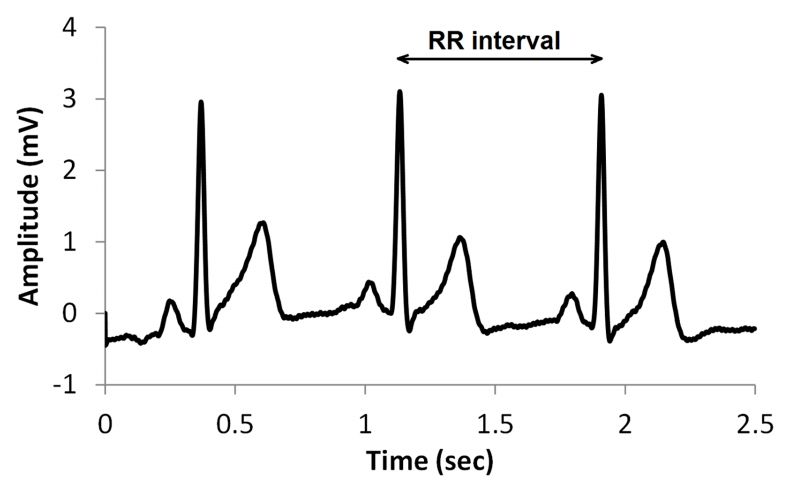
\includegraphics[keepaspectratio=true, width=0.4\textwidth]{./rr_example.jpg}
 \caption{A typical ECG signal showing the RR interval.}
\label{fig:example_rr_interval}
\end{figure*}


\subsection{Data Analysis}

\subsubsection{Cluster Analysis of Motion Data}

R-R series were divided into episodes (epochs) based on accelerometer data. Sections of acceleration time series representing similar activities were determined and such partitioning was used to extract R-R epochs directly. This approach allowed us (1) to determine the R-R epochs recorded during consistent conditions (one particular type of activity) and (2) to group the R-R series according to these conditions (movement types). The accelerometer data was classified using cluster analysis.

Cluster analysis (or clustering) is a data mining technique grouping a set of objects in such a way that objects in one group (called \textit{cluster}) are more similar to each other than to the objects in other groups. Clustering of time series data enforces the usage of indirect feature extraction methods (see survey~\cite{timeseriesclustering_survey} for general introduction in the subject). The most straightforward approach involves computing a \textit{sliding window} over the time series (i.e. a fixed-size subset of consecutive elements of time series) and composing a feature (or observation) vector using simple statistics that convey general information about a particular window. This approach is commonly used for human activity classification using accelerometer data~\cite{bao2004activity, AMT_towards}. For a review of different techniques see~\cite{altun2010comparative} and for comparison of various sensor mounting positions see~\cite{atallah2011sensor}. Reference dataset for firefighting activity recognition is described in~\cite{meina2015tagging}.

In this study cluster analysis was performed on a motion data time series of length $T$ obtained from the sensor:
\begin{equation}
    \mathbf{a}_t := (a_t^{lat}, a_t^{lon}, a_t^{ver}), \quad \mbox{for} \enspace t \in \{1, 2, 3, \ldots, T\},
\end{equation}
where each element of the series~$\mathbf{a}$ was a measurement of an acceleration given at time $t$ of the sensor's frame of reference. Due to the position of the sensor's mounting points, when the subject remained upright, values $a^{lat}$ and $a^{lon}$ represented the two components of acceleration along the lateral and longitudinal axes, respectively, in the plane parallel to the surface of the Earth, while $a^{ver}$ approximated acceleration along the vertical axis, in the plane perpendicular to the surface of the Earth. A real-life example of such motion data time series containing all three acceleration components can be found in the bottom plot of Fig.~\ref{fig:example_clustering} (the subject remained in an upright position throughout most of the day, whereas between $\sim$11\,p.m.\ and $\sim$7\,a.m.\ the subject was sleeping in a horizontal position).

Clustering analysis was performed on short subsequences of the data, defined formally as a \textit{sliding window} $W$ of length $m$ at time $t$:
\begin{equation}
    W_m(t) := [\mathbf{a}_{t - m}, \ldots, \mathbf{a}_{t - 2}, \mathbf{a}_{t - 1}, \mathbf{a}_t ],
\end{equation}
where $t = m + 1, \dots, T$.
The $r$-dimensional feature vector was computed using a set of simple statistical functions (i.e. $\max$, $\min$, variance, mean, median and kurtosis) over the sliding window:
\begin{equation}
    \mathbf{x}(t) := \big[ f_1(W_m(t)), \ldots, f_r(W_m(t)) \big],
\end{equation}
where $t = m + 1, \dots, T$, and $f_j$ is one of the statistical functions listed above.

Subsequently, the $k$-means clustering technique was used~\cite{kmeans}. This method aims to find a partition of all observations into $k$ disjoint sets $C := C_1 \cup C_2 \cup \ldots \cup C_k$ ($C_i \cap C_j = 0; i,j<k$) resulting in a minimized within-cluster sum of squares ('similarity' of feature vectors):
\begin{equation}
    \argmin_{C} \sum_{i = 1}^{k} \sum_{x \in C_i} \|x - \mu_i\|^2,
\end{equation}
where $\mu_i$ is the {\em centroid\/} of cluster $C_i$, equal to the mean of all points in cluster $C_i$.

Due to the abundance of data, mini-batch $k$-means described in~\cite{minibachkmeans} method was applied. Sliding window size ($m$ parameter) was chosen to extract the longest possible consistent episodes at the value of $m=500$ which corresponds to 2[s] of data. From the evaluation~\cite{windowSize}, the interval 1-2 s proves to provide the best trade-off between recognition speed and accuracy. Clustering was followed by majority interpolation with a moving window of 30[s] -- this procedure eliminates noisy classification regardless of window size.
% * <jezu.febsu@gmail.com> 2017-11-12T21:22:01.061Z:
%
% > majority
% by a major /?/
%
% ^.



% Figure~\ref{fig:example_clustering} pokazuje przyklad calodziennego nagrania danych z pasa Equvital zebranego od jednego z uczestnikow badania. Jak widac zostalo wydzielone 45 episodow (grup) (10 roznych). Podczas calodzinnego nagraia strazak uczestniczyl w cztereg wyjazdach co zostalo oznaczone przez box w dolnym wykresie.
Partitioning of motion data representing human physical activity is ambiguous due to no sharp predefined cut-off points between different types of activity. For example: there certainly is a clear difference between walking and running, but data recorded in the non-laboratory environment may contain representations of several intermediate gait styles and other vaguely defined kinds of locomotion. Moreover, creating a precise and understandable description of various activities is very challenging (not to mention the costs of data annotation). Therefore, it is much more convenient to use the concept of 'similarity' of activities.

%This  Attempts to classify gait and outline the affecting factors can be found in literature, e.g.~\cite{levine2012whittle}.

Since it is so difficult to predefine a theoretical number of movement types, in this study we have considered several different clustering scenarios. Since the $k$-means algorithm makes it possible to preset a fixed $k$-parameter of the centroid, clustering was performed for a various number of clusters $k = 10, 15, 20$ and $25$.

\subsubsection{HRV analysis}

Heart Rate Variability analysis was performed using standard methods implemented in RHRV, an open-source package for the R environment. HRV measures were calculated from epochs of the R-R interval time series, delineated in two subsequent steps. 1) First, the endpoints of R-R epochs were based on the time frames of the previously defined clusters of motion data, which can be understood as episodes of different types of movements. Such analytical design allowed us to compare HRV metrics for all subjects divided into separate clusters, i.e.\ during \textit{different activities (physical effort)}. 2) Next, R-R epochs created in the first step were divided further with the use of information about the time frames of the emergency incidents, seen as episodes of increased stress. The second step enabled us to compare HRV metrics for all subjects within a given cluster, but between different physiological load, i.e. during  (\textit{similar activities (physical effort)}) under \textit{different amount of stress} (incident \textit{vs.} no incident).

%Analiza zmienności rytmu zatokowego została dokonana używajac standardowych metod (zaimplementowanych w RHRV, an OpenSource package for the R environment). Episody brane pod uwage były wygenerowane okreslone przy użyciu grup. Innymi słowy poszczególna grupa stworzona na podstawie danych kinematycznych posłużyła do wyznaczenia odcinków czasowych w szerego R-R,

HRV indices were calculated using linear methods in time domain (SDNN, SDANN, SDNNIDX, pNN50, SDSD, rMSSD, IRRR, MADRR, TINN, HRVi), and non-linear methods, such as Poincar\'e plot (SD1, SD2) and entropy measurements (Correlation Dimension, $D_2$, and Scaling exponent, ScalExp) (for description of HRV parameters applied in this study see: Table~\ref{tab:hrv_ann}). Time-domain analysis is well grounded in psychophysiological research, and the indices calculated reflect the functioning of the sympathetic and parasympathetic branches of the autonomic nervous system~\cite{berntson1997heart}. Physiological connotations of non-linear dynamics are less well understood; however, the calculated measures appear very sensitive in discriminating various psychophysiological states~\cite{sassi2015advances,young2015we}.

Detailed description of used metrics is enclosed in Tab.~\ref{tab:hrv_ann}.

\begin{table*}[ht]
\begin{adjustwidth}{}{0in}
\caption{HRV analysis parameters. Hereafter, NN refers to 'normal-to-normal' beats of the heart, equal to RR, i.e. peak-to-peak period between the R-waves on the ECG.}
\label{tab:hrv_ann}
\begin{tabular}{lp{0.77\textwidth}}
\hline
HRV index & Description \\
\hline
SDNN & Standard deviation of the inter-beat NN (RR) intervals \\
SDANN & Standard deviation of the NN (RR) intervals averaged over 5-minute periods \\
SDNNIDX & Mean value of SDNN \\
pNN50 & Proportion of the adjacent (successive) NN (RR) intervals greater than 50\,ms \\
SDSD & Standard deviation of the successive differences between the adjacent NN (RR) intervals \\
rMSSD & Root mean square differences between the successive NN (RR) intervals \\
IRRR & Length of the interval between the first and the third quantile of the $\Delta$RR time series \\
MADRR & Median of the absolute values of the successive differences between the adjacent NN (RR) intervals \\
TINN & Triangular interpolation of the NN (RR) interval histogram. \\
HRVi & Index reflecting the slowing down of the heart \\
SD1 & Dispersion of the points along the minor axis of the Pointcare plot (SD of the short-term RR-interval variability) \\
SD2 & Dispersion of the points along the major axis of the Pointcare plot (SD of the long-term RR-interval variability)\\
$D_2$, ScalExp & Non-linear dynamics measures of time series \\
\hline
\end{tabular}
\end{adjustwidth}
\end{table*}

\subsection{Statistical analysis}
Stress self-assessment data was analyzed in SPSS statistical software. Results for cadets and professionals were compared with a Student's t-test, following a variance homogeneity check performed with a Levene's test.

Statistical analysis of physiological data was performed in the R software package. Due to the fact that emergency incidents constituted only a small part of the daily schedule, far less data were collected during action than during non-action activities. Moreover, it is very likely that certain types of activities are not present during incidents. Therefore, due to the disproportion in sample sizes (action vs. non-action), mean values of HRV indices were compared between incident and non-incident with a Welch's $t$-test. Our hypothesis concerns the possibility of separating incident from non-incident situations within a particular cluster based purely on HRV metrics.

For the statistical analysis involved in machine learning and classification, Python packages \textit{sklearn} and \textit{seaborn} were used. Test data consisting of random R-R epochs were evaluated as "incident" or "non-incident" upon binary classification with a Na\"{i}ve Bayes classifier. The evaluation was based on a ROC Analysis performed on the averaged classification result, using stratified shuffle splitting with 300 folds (due to the highly unbalanced data).

\section{Results}

\subsection{Self-assessment of Perceived Stress}

A total of N = 43 emergency incidents were recorded (23 for cadets and 20 for professional firefighters). In most cases the answers indicated that the subjects experienced mild stress or no stress at all. Only a few emergency incidents were marked as stressful, while most were assessed as very routine, typical interventions. Mean answers and their standard deviations were summarized for each question and for the whole questionnaire in Table~\ref{tab:stress_quest}. The self-assessment results suggested there was very little stress experienced by the firefighters during fire incidents. The total score did not show normal distribution, and exhibited a skew towards lower values (skewness 0.849). In the range of theoretical minimum of 11 pts and maximum of 55 pts, the median answer was 22 pts with a min-max range of 13-38 pts.
Mean total score did not differ between cadets and professional firefighters (t=0.36(38.6), p=.718). However, professionals reported higher perceived stress (question no. 1; t=-3.00(34.6), p=.05), but also higher self-satisfaction (question no. 10; t=-2.23(41), p=.032) than cadets.
Information about the emergency incidents was retrieved from an open question: "In a few short sentences, characterize the situation and your feelings about it (state the type of action, equipment used, difficulties encountered in action, victims/injured parties [people, animals and possessions], and any information that seems important to you)". Quality analysis of the answers revealed that the majority of the  emergency incidents recorded were grass fires, minor city incidents and trainings, and only a few were serious events, such as a burning building.

\begin{table*}[ht]
%\begin{adjustwidth}{-2.25in}{0in} % Comment out/remove adjustwidth environment if table fits in text column.
\caption{Results of self-assessment of stress with a questionnaire. Mean and SD calculated for each question and total score.}
\label{tab:stress_quest}
\centering
%\begin{tabular}{lp{0.8\textwidth}}
\begin{tabular}{lp{0.7\textwidth}ll}
\hline
No. & Question & Mean & SD \\
\hline
1. & To what degree was the situation stressful to you? & 1.91 & 0.75 \\
2. & To what degree was the situation \textbf{not} a challenge to you? & 3.56 & 1.03 \\
3. & To what degree was the action routine? & 3.60 & 1.20 \\
4. & To what degree was the situation a threat to your life? & 1.47 & 0.74 \\
5. & Did the situation endanger civilians in your surroundings? & 1.84 & 1.15 \\
6. & To what degree did the situation endanger other firefighters involved in the action? & 1.44 & 0.73 \\
7. & To what degree was the situation \textbf{not} a threat? & 3.77 & 1.25 \\
8. & Assess the amount of effort you had to undertake in this situation & 2.16 & 0.92 \\
9. & Was your involvement crucial to the action? & 2.81 & 1.16 \\
10. & Assess how satisfied you are with your actions during the incident & 3.77 & 0.81 \\
11. & Assess how satisfied you are with your co-operation with other participants throughout the action & 4.12 & 0.66 \\
% reverse questions: 2, 3, 7, 10, 11
\hline
 & Total score & 22,81 & 5,36 \\
\hline
\end{tabular}

\footnotesize
Rated on 5-point Likert-type scale: ranging from strongly disagree (1) to strongly agree (5)
%\end{adjustwidth}
\end{table*}

\null
\subsection{Physiological recordings}
A total of 26 sets of 24h recordings of physiological data were gathered, and following initial data quality inspection, 25 sets were accepted for further analysis. The whole data set consisted of 485\,h of recordings, out of which 45\,h 15\,min were recorded during 39 fire incidents. Data were collected on duty while subjects were performing different types of activities. 17 subjects were involved in some kind of incident (9 cadets and 8 professionals). The attended fire incidents were reported by the firefighters to had lasted varying amounts of time (17\% was $<$18\,min, 52\% $<$43\,min, 87\% $<$85\,min). One incident was annotated as 6\,h long.

\subsection{Clusters of acceleration data}

Cluster analysis is an unsupervised learning method and therefore, could not provide an explanation of the kind of activity corresponding to a particular cluster, but facilitated grouping the analyzed motion data into clusters of similar activities. In this way, a given movement recorded from one subject is more similar to another of their movements grouped into the same cluster, or even to a movement performed by a different subject but still within the same cluster, than to any of their or others' movements grouped into a different cluster. This allows to group together similar episodes of accelerometer data and delineate types of activity differing with respect to motion parameters, however, without labeling them.

Figure~\ref{fig:example_clustering} shows an exemplary recording from one of the participants, separated into 84 episodes grouped into 20 clusters. During the time of the recording, the firefighter participated in four emergency incidents marked by gray boxes.

\begin{figure*}[ht!]
 \centering
 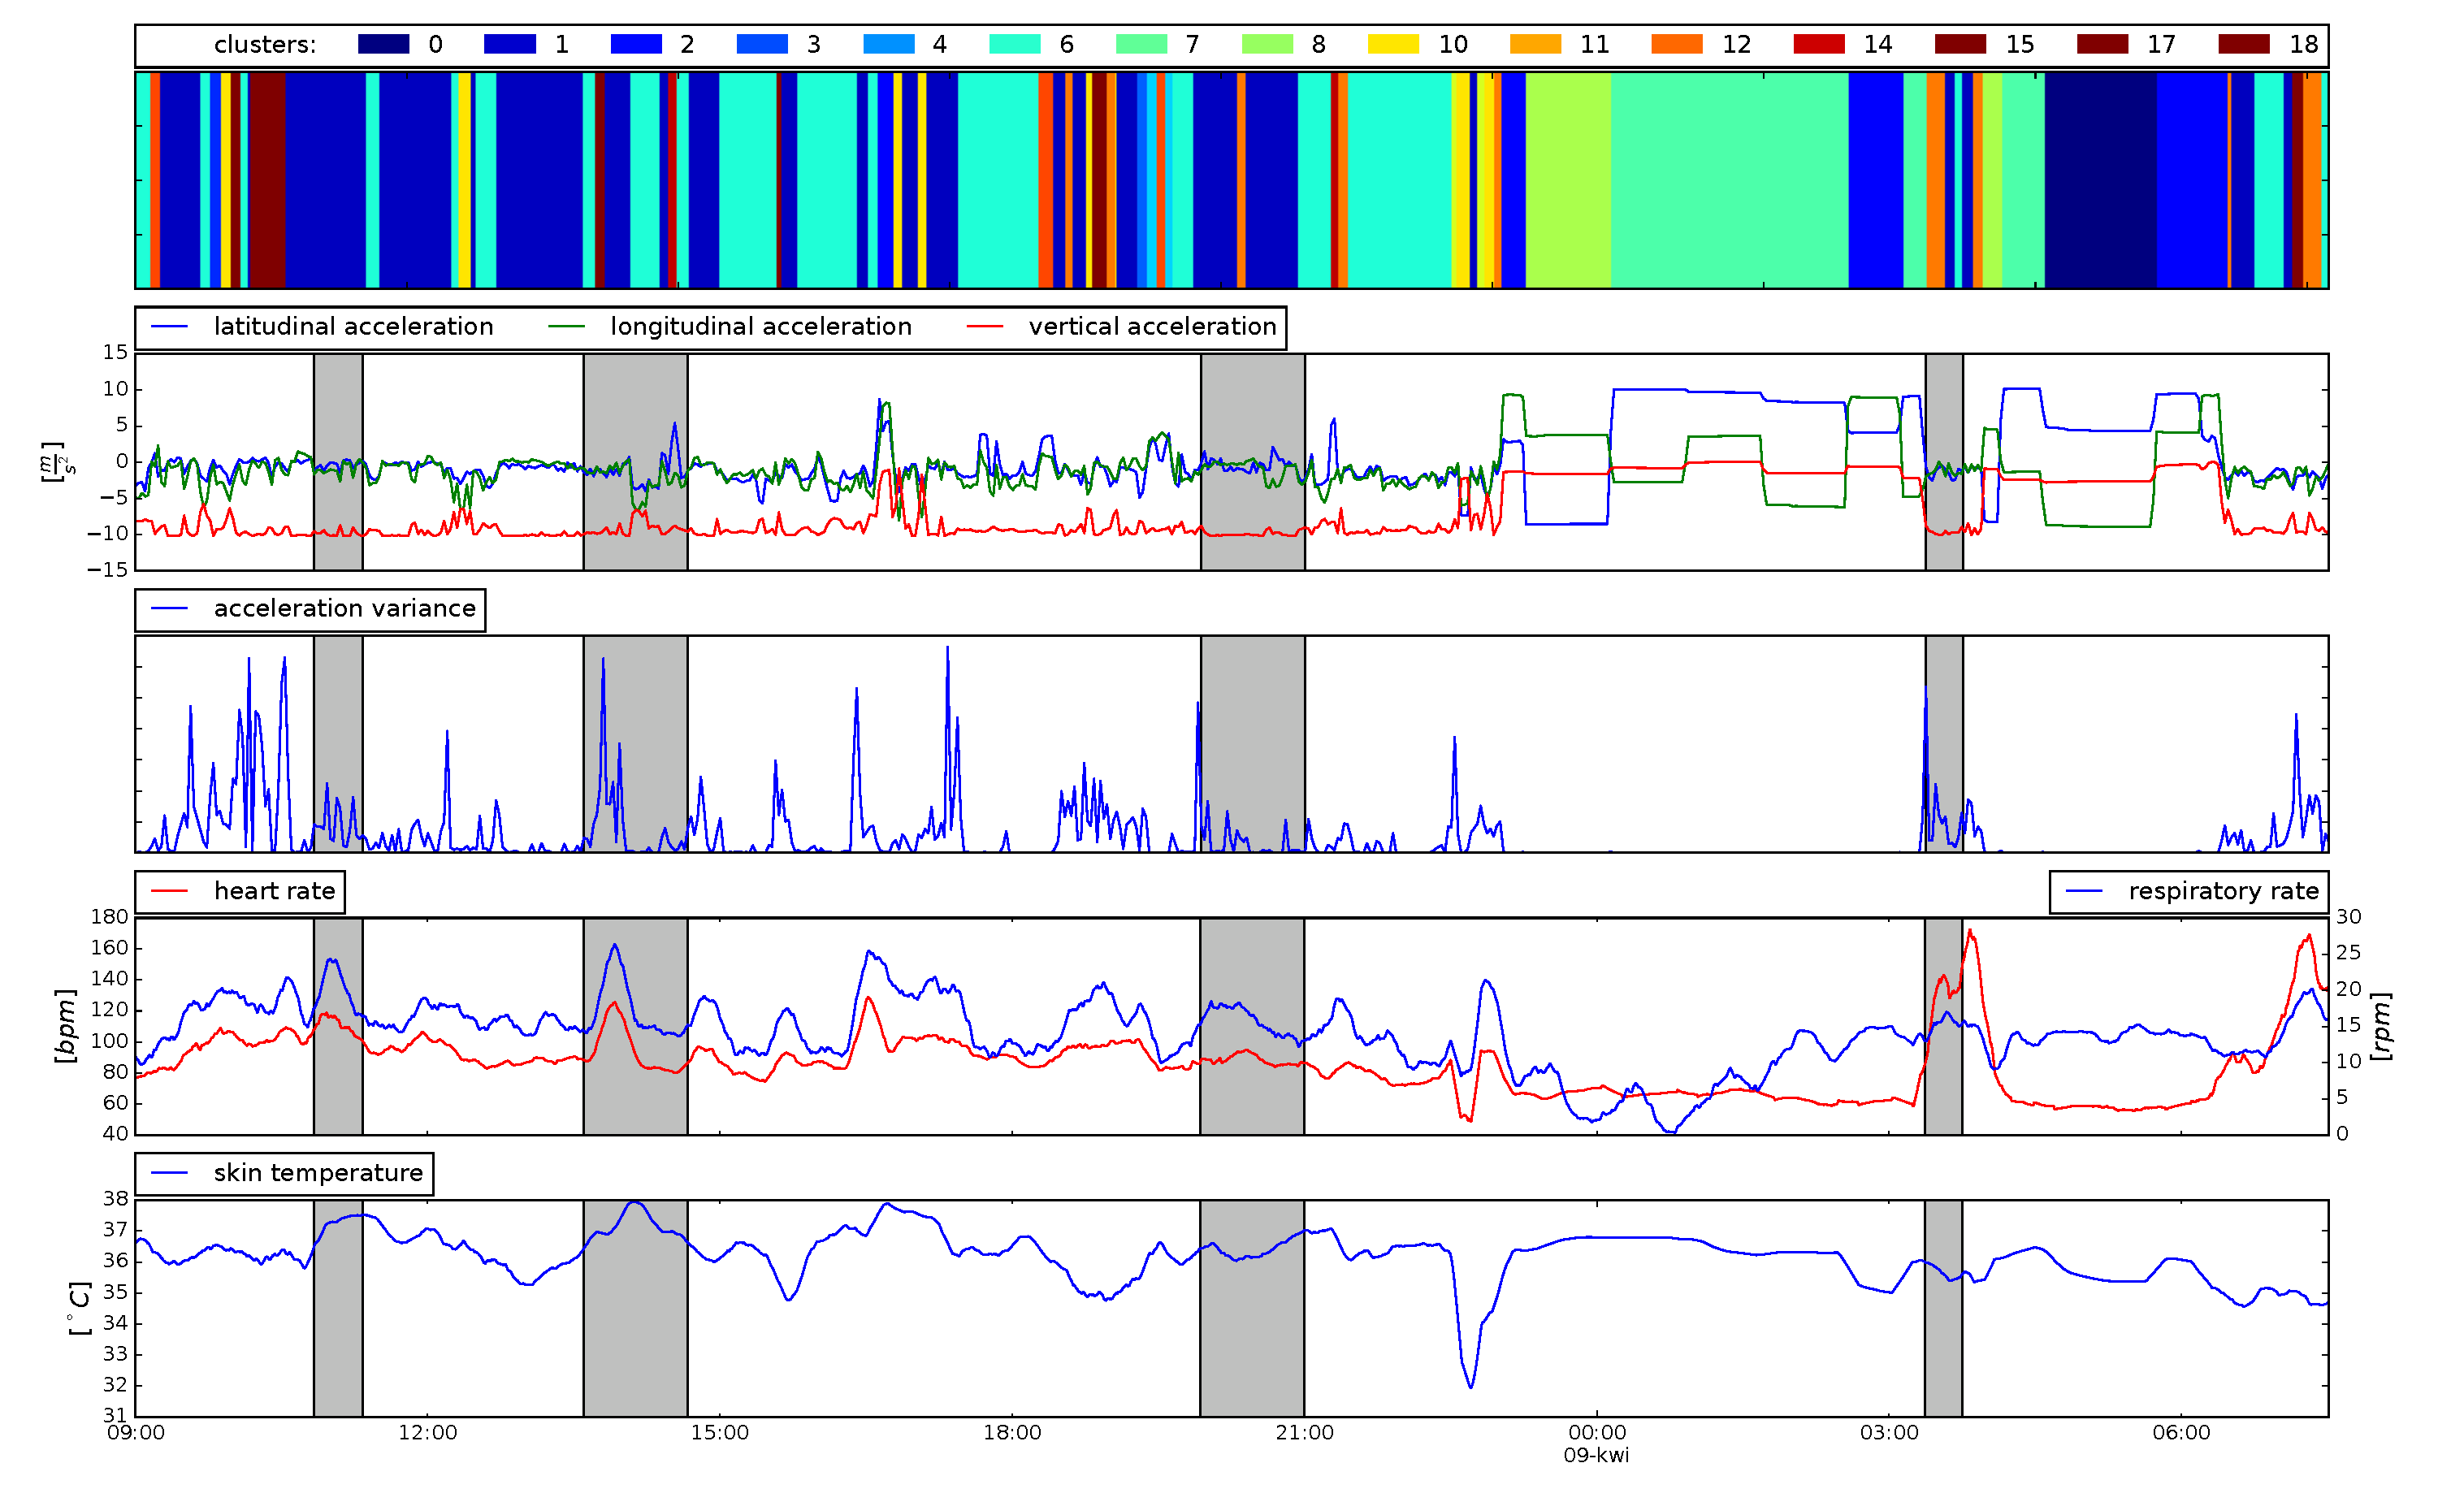
\includegraphics[keepaspectratio=true, width=\textwidth]{./clustering_example.eps}
 % clustering_example.pdf: 720x216 pixel, 72dpi, 25.40x7.62 cm, bb=0 0 720 216
 \caption{Exemplary data from a 24h recording retrieved from one of the participants. Consecutive graphs (marked by the successive letters of the alphabet) correspond to the same time-line. Figure 1a. depicts clusters of motion time series. Motion data consists of three-axial acceleration measurements, and acceleration variance, presented in Figure 1b. and 1c., respectively. Figure 1d. illustrates changes in HRV (red line, left axis) and respiration rate (blue line, right axis), while 1e. shows fluctuations in body temperature.}
\label{fig:example_clustering}
\end{figure*}


The immediate observation from Fig.~\ref{fig:example_clustering} is that the peeks of acceleration variance are connected with different clusters, which can be  understood as high intensity and low-intensity movements. Around 11PM we can observe long episodes of resting, where only few clusters are depicted (no. 3, 7, 8) – the ones that are not present during the day and correspond to a different position of the subject. It is very interesting to note that the respiratory and heart rates increase during incidents as well as during normal activities. Around 10PM we see a sudden drop of the temperature connected with temporary sensor dismounting.


Prior to HRV analysis between incident and non-incident, signal partitioning was controlled for incorrect classification \textit{indirectly} based on the HRV metrics; a situation, when clustering is influenced by its own methodology and therefore not reliable. We identified two theoretical instances when such a problem could occur: (1) when the incident is present in only one or two clusters, and (2) when epoch length affects HRV metrics. The former situation indicates that classification of R-R episodes as 'action' is based on the presence of a very specific type of activity, occurring \textit{only} during incidents. However, in our study, 4 clusters were found to contain both 'action' and 'no action' episodes. Considering the latter case, the highest correlation between episode length and HRV value observed in our study was $.22$ ($p<.01$, Spearman rank correlation) for SDANN. Despite the fact, that this correlation was weak, the SDANN metric was nonetheless rejected from further analysis. Logistic regression confirmed that cluster number \textit{did not} predict attribution to an emergency incident ('action'). Therefore, we assume that clustering alone did not carry significant information about the incidents. Some clusters did not contain any data form the emergency incidents, however, that is easily explainable by the specificity of motion represented by a given cluster. For example, certain clusters contained large fractions of data where the subject remained in a stationary, horizontal position (most probably sleeping), that (hopefully) did not occur during the incident. In the clusters reflecting an emergency event, data proportion of incident/non-incident recordings was consistent with the overall data.

\subsection{Classification of R-R episodes}

Location test was performed on different HRV metrics computed over R-R episodes delineated according to motion data clustering with parameter $k=10$. In 6 out of 10 clusters, less than 2 incident events were present, excluding these clusters from analysis. In the remaining 4 cases, incident events constituted on average 8\% of all episodes within a cluster.

Results of a Welch's $t$-test revealed differences in the average of different HRV metrics between 'incident' and 'non-incident' situations. Additionally, considering partitioning of episodes by physical activity, these situations could be distinguished in overall data-set but not necessarily for individual episodes.  Standard deviations of HRV metrics within the final partitioning are high; however, in most cases a tendency of lower mean HRV upon 'incident' can be noted. Interesting fact is that in one cluster (no 8) the mean tendency is reversed. Tab.~\ref{tab:location_test_result} summarizes the results of location test for different HRV metrics along with the corresponding means and standard deviations.

\begin{table*}
\caption{The result of mean equality test between different HRV metrics divided into motion clusters. Only clusters on which a location test was done (due to the sufficient number of incident events)}
\label{tab:location_test_result}
\setlength{\tabcolsep}{5pt}
\begin{tabular}{rllll}
\hline
& \multicolumn{4}{c}{ClusterID (incident/non-incident episodes)} \\
&    1 (25/166)    &    2 (3/48)    &    6 (11/151)    &  8 (5/126)) \\
\hline
SDNN [ms]       &    .312          &    .608        &    .203        &    .271 \\
  incident     & 117.92 $\pm$ 41.52   & 83.47 $\pm$ 35.30  & 112.12 $\pm$ 50.22 & 98.96 $\pm$ 27.27 \\
  non-incident & 128.61 $\pm$ 65.50   & 107.45 $\pm$ 48.97 & 134.62 $\pm$ 64.33 & 27.27 $\pm$ 56.94 \\
\rule{0pt}{3ex}
SDNNIDX [ms]   &    .166          &    .522        &    .050**        &    .083 \\
  incident     & 93.52	  $\pm$  46.06   &   74.73  $\pm$ 43.20   &  99.24  $\pm$ 50.84   &   76.68  $\pm$ 19.02 \\
  non-incident &  104.52	$\pm$  59.65   &   95.65  $\pm$ 47.51   &  110.80 $\pm$ 60.70   &   19.02  $\pm$ 54.30 \\
\rule{0pt}{3ex}
pNN50 [\%]       &    .225          &    .735        &    .084        &    .018** \\
  incident     & 18.61	  $\pm$  13.89   &   11.88  $\pm$ 11.45   &  15.92  $\pm$ 14.29   &   13.99  $\pm$ 9.53		 \\
  non-incident & 23.30   $\pm$  16.05   &   22.21  $\pm$ 14.17   &  26.36  $\pm$ 16.81   &   9.53   $\pm$ 16.58 \\
\rule{0pt}{3ex}
SDSD [ms]          &    .225          &    .735        &    .084        &    .018** \\
  incident     & 65.00	  $\pm$  44.10   &   61.43  $\pm$ 47.03   &  60.93  $\pm$ 47.39   &   44.16  $\pm$ 16.89		 \\
  non-incident & 78.71   $\pm$  58.71   &   81.26  $\pm$ 47.61   &  92.33  $\pm$ 61.78   &   16.89  $\pm$ 48.14 \\
\rule{0pt}{3ex}
rMSSD [ms]     &    .308          &    .471        &    .447        &    .106 \\
  incident     & 64.98	  $\pm$  44.08   &   61.41  $\pm$ 47.01   &  60.92  $\pm$ 47.37   &   44.15  $\pm$ 16.88		  \\
  non-incident & 78.65   $\pm$  58.54   &   81.17  $\pm$ 47.55   &  92.22  $\pm$ 61.52   &   16.88  $\pm$ 48.12 \\
\rule{0pt}{3ex}
IRRR [ms]          &    .173          &    .607        &    .020**        &    .069 \\
  incident     &  151.52	$\pm$  63.06   &   80.00  $\pm$ 37.00   &  154.00 $\pm$ 97.90   &   115.00 $\pm$ 18.11		 \\
  non-incident &  168.31  $\pm$  110.14  &   120.23 $\pm$ 74.10   &  177.93 $\pm$ 117.43  &   18.11  $\pm$ 85.11\\
\rule{0pt}{3ex}
MADRR  [ms]        &    .991          &    .793        &    .922        &    .882 \\
  incident     & 20.64	  $\pm$  12.09   &   14.00  $\pm$ 10.00   &  16.27  $\pm$ 11.28   &   18.00  $\pm$ 8.17		 \\
  non-incident & 25.16   $\pm$  17.99   &   20.84  $\pm$ 12.91   &  26.52  $\pm$ 16.03   &   8.17   $\pm$ 18.49 \\
\rule{0pt}{3ex}
TINN [ms]         &    .991          &    .793        &    .922        &    .882 \\
  incident     & 335.49	$\pm$  98.45   &   214.78 $\pm$ 102.79  &  315.20 $\pm$ 80.28   &   311.77 $\pm$ 23.04		 \\
  non-incident &  333.28	$\pm$  136.37  &   243.49 $\pm$ 105.54  &  306.71 $\pm$ 105.84  &   23.04  $\pm$ 144.73 \\
\rule{0pt}{3ex}
HRVi           &    .225          &    .735        &    .084        &    .018** \\
  incident     & 21.47	  $\pm$  6.30    &   13.75  $\pm$ 6.58    &  20.17  $\pm$ 5.14    &   19.95  $\pm$ 1.47		 \\
  non-incident & 21.33   $\pm$  8.73    &   15.58  $\pm$ 6.75    &  19.63  $\pm$ 6.77    &   1.47   $\pm$ 9.26 \\
\rule{0pt}{3ex}
SD1  [ms]          &    .331          &    .576        &    .246        &    .367 \\
  incident     & 45.96	  $\pm$  31.18   &   43.43  $\pm$ 33.25   &  43.09  $\pm$ 33.51   &   31.23  $\pm$ 11.94		 \\
  non-incident & 55.65   $\pm$  41.51   &   57.46  $\pm$ 33.66   &  65.29  $\pm$ 43.68   &   11.94  $\pm$ 34.04 \\
\rule{0pt}{3ex}
SD2  [ms]          &    .008*         &    .648        &    .121        &    .021 \\
  incident     & 159.42	$\pm$  52.28   &   108.34 $\pm$ 41.15   &  151.51 $\pm$ 65.12   &   136.26 $\pm$ 37.24		 \\
  non-incident & 172.22  $\pm$  84.50   &   139.49 $\pm$ 62.37   &  177.44 $\pm$ 82.81   &   37.24  $\pm$ 74.53 \\
\rule{0pt}{3ex}
$D_2$          &    .010*         &    .400        &    .095        &    .296 \\
  incident     & 1.44    $\pm$  0.06    &   1.25   $\pm$ 0.13    &  1.43   $\pm$ 0.04    &   1.46   $\pm$ 0.02		 \\
  non-incident & 1.35    $\pm$  0.33	   &   1.28   $\pm$ 0.35    &  1.39   $\pm$ 0.21    &   0.02   $\pm$ 0.15 \\
\rule{0pt}{3ex}
ScalExp        &    .157          &    .767        &    .053        &    .015 \\
  incident     & 1.01    $\pm$  0.11    &   1.19   $\pm$ 0.22    &  1.07   $\pm$ 0.20    &   1.05   $\pm$ 0.19		 \\
  non-incident & 0.91    $\pm$  0.21	   &   0.86   $\pm$ 0.29    &  0.92   $\pm$ 0.25    &   0.19   $\pm$ 0.23 \\
\hline
\end{tabular}
\end{table*}

Additionally, means of all HRV indices were compared between clusters with a one-way ANOVA, showing significant differences ($p<.001$) for  SDANN, IRRR, TINN, HRVi, SD2, and CD. A post-hoc pairwise test raveled that most often significant differences occurred for clusters 2 \textit{vs.} 6, and 1 \textit{vs.} 2, accordingly.

Best results of  individual R-R episode classification as 'incident' or 'no incident' was achieved with AUC score of $.7$ ($.65$ for feature set without information on cluster number).  More granular clustering (higher k-parameter) decreased the classification accuracy. Ranking the HRV metrics by Information Gain slightly improved the classification score. Final feature set composed of the following metrics: ClusterID, ScalExp, pNN50, MADRR, IRRR, HRVi, CD. Fig.~\ref{fig:ROC_curve} summarizes the classification results.

\begin{figure*}[htbp!]
 \centering
 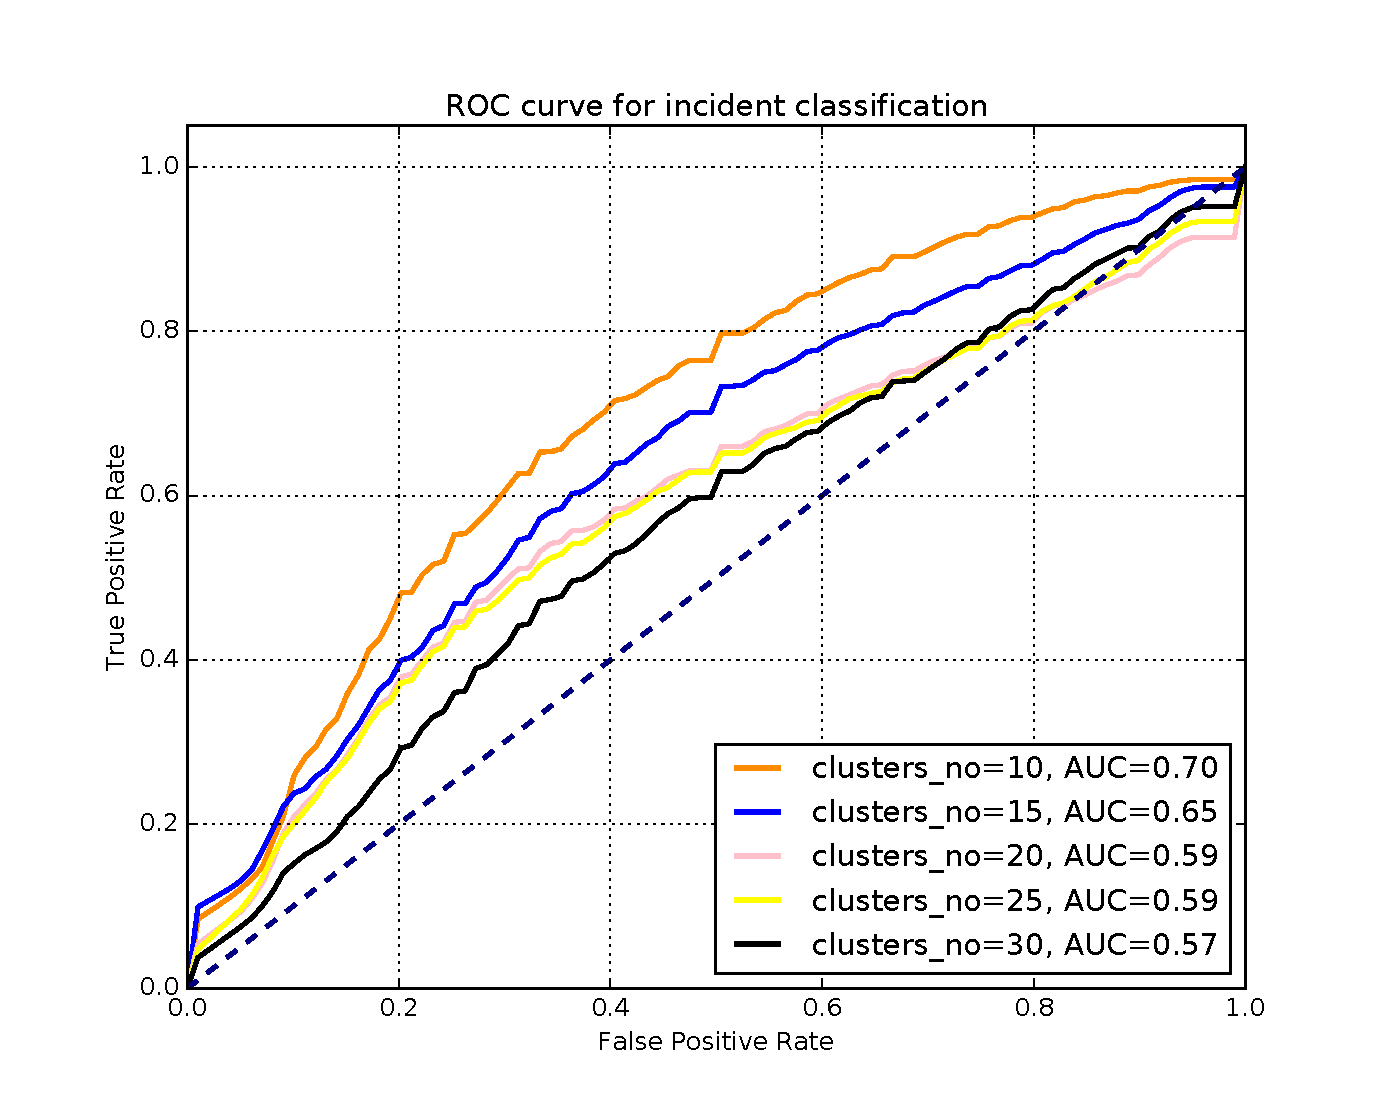
\includegraphics[keepaspectratio=true, width=0.7\textwidth]{roc_analysis.eps}
 \caption{Classification for incident detection using HRV metrics performed on R-R epochs induced by different clustering parameters ($k=10,15,20$ and $25$) applied to accelerometer data}
\label{fig:ROC_curve}
\end{figure*}


\section{Discussion}

\subsection{Outcomes and applications}

In this study, motion data was collected throughout a 24-hour day of work together with corresponding HRV readings. With the use of machine learning techniques, physiological data (R-R series) was subjected to automatic binary classification, indicating whether given data was recorded during or outside of an incident. The best results were achieved for data separation performed by clustering of motion data (Fig.~\ref{fig:ROC_curve}), based on motion parameter vectors constructed with acceleration values. This approach allowed separation of events varying in physical activity into separate clusters. Each epoch of the R-R series analyzed was tagged as ‘incident’ or ‘no incident’ in accordance with information about the presence/absence of an emergency incident. It was assumed that ‘incident’ equaled 'stress', while ‘no incident’ was a situation of 'no stress'. Not all of the motion clusters were represented during an emergency situation. This is understandable when considering different types of physical activity, such as sleeping/lying motionless, which, for obvious reasons, do not appear during incidents. For 4 out of 10 clusters separated into the  ‘incident’ and ‘no incident' (‘stress’ and ‘no stress’) sub-groups, various HRV indices were compared Tab.~\ref{tab:location_test_result}. For each cluster only one or two indices showed statistically significant differences in mean HRV between sub-groups. This is probably due to the high variance and unequal sample sizes between the compared partitioning. Fire incident emergencies contributed to a small percentage of the firefighters’ daily activities. Therefore, the ‘stress’ group was underrepresented with respect to the ‘no stress’ group, which contained many more episodes. Also, different HRV metrics distinguished the 'stress'-'no stress' conditions within each of the analyzed clusters (SD2 and D2 in cluster 1, IRRR and SDNNIDX in cluster 6, and pNN50, SDSD, HRVi, SD2 and ScalExp in cluster 8). This might be due to different sensitivity of the indices, to HRV change in general, as some reflect activity of the sympathetic branch of the autonomic nervous system, some – of the parasympathetic branch, and others – of both, or the balance between the functioning of the two~\cite{task1996heart,sassi2015advances}. However, such a situation could be caused by various reaction of HRV metrics to a specific behavior of the cardiovascular system exhibited during a particular type of motion (represented by a given cluster) and/or different sensitivity to stress-induced change in HRV (within that cluster).

Nevertheless, the general trend was as expected, with lower HRV values upon stressful situations. Previous studies reported the usefulness of HRV data as a psychophysiological marker of stress~\cite{pereira2017heart}. However, in our study we confirmed that HRV parameters can distinguish stressful situations in ecological settings, and the results achieved correspond to the outcomes of studies in laboratory settings. Studying stress in a natural environment leaves no control over exact timing and amount of stress experienced by the subjects. This fact may be reflected in the lower statistical significance of differences in mean HRV values between ‘stress’ and ‘no stress’ situations. Nevertheless, these results still reflect the outcomes of carefully planned experiments in artificial settings, only to a lesser extent. This study confirms that HRV indices are robust psychophysiological indicators of stress beyond the laboratory, in ecological conditions.

%Physiological data – both accelerometric and HRV parameters – was subjected to machine learning with 300 folds of random data selection into learning set and test set. Addition of HRV values calculated from time series corresponding to the delineated motion episodes allowed to further increase clusterization specificity. Data was classified into ‘stress’ (emergency action) and ‘no stress’ sub-clusters.
%Analysis of the confusion matrix shows that about 1 in 6 accidents and 1 in 33 non-accidents are classified correctly.

ROC curve analysis showed that appropriate decision criteria allowed to classify 15\% of incidents with no false alarms, which may seem to be a huge underestimation. However, the results of the self-assessment stress questionnaire showed that only a few emergency actions had been evaluated by the participants as moderately stressful. Only in 14\% of the reports (6 out of 43) the answer to Question 1. ‘To what degree was the situation stressful to you?’ was rated as 3 or more on the Likert scale. Considering these findings, the 15\% true positive may represent the ~\textit{actual} amount of stressful incidents. These results show a good correspondence between the psychometric and physiological data, allowing us to rely on psychophysiological parameters as indicators of stress.

Results obtained in this study indicate that during their everyday service, the firefighters experienced low-to-moderate stress, and most emergency incidents were highly routine. The total score of a self-assessment questionnaire of experienced stress showed no statistically significant differences between fire school cadets and professional firefighters. However, professionals seemed to perceive more stress, but also more satisfaction from their job. Since these two groups belonged to two different fire departments, it is most likely that this result simply reflects the differences in particular emergency incidents attended by both groups. However, it is also possible, that the cadets were given less demanding tasks during action, or that they were underestimating the stress perceived in order to present a particular self-image (reporting lower stress attributed to being ‘strong’ and ‘tough’). Moreover, low overall stress assessment score may represent seasonal specificity of incidents (the recordings took place during summer season, which is perceived as uneventful).

%TO ZDANIE JEST NIEPOTRZEBNE: During summer season, when data was collected, mostly grass fires are reported, which are rated as low-danger incidents. The firefighters admitted that winter season is far more stressful, when coal ovens in low-budget households cause dangerous fires or carbon monoxide poisoning, resulting in civilian victims and much more demanding emergency actions.

Additionally, the firefighters reported to usually experience the strongest agitation before the beginning of an emergency intervention. The moment of receiving dispatch instructions and departing for action was indicated as very stressful, while once the situation recognition is over, routine action and typical behavior allows for good control and planning, resulting in decreased stress. Following an emergency incident, firefighters report low stress and life threat on action. Therefore, the initial psychophysiological activation is taken into account neither in post-action debriefing nor in self-assessment psychometric questionnaires. It appears that self-reporting of stress remains non-discriminative and non-informative in this matter. Therefore, the nature of chronic, everyday stress experienced by the firefighters may remain neglected, despite the fact that it is inherent to the profession. Strong, acute stressors occur with various frequency; however, chronic stress accompanies high-risk professionals throughout their career on a daily basis. The inability to control and predict the outcome of a difficult and/or life-threatening situation results in a frequent mobilization of the sympathetic branch of the autonomic nervous system. Experiencing chronic stress leaves insufficient time for the system to return to a balanced state, leading to the development of affective and other stress-related disorders. It is therefore crucial to monitor levels of chronic stress experienced by employees, especially in high-risk jobs, such as firefighter service. Physiological monitoring may be very informative in this matter, providing objective, yet personalized and very detailed information about the daily profile of experienced stress.

These findings may suggest practical implementations. The same clusters were present in data profiles of different subjects. Therefore, clusters can be considered universal and independent of individual characteristics of movement styles and HRV. In theory, it would be possible to assign tags (‘names’) to each delineated cluster. Therefore, it seem possible to construct a universal classifier, that could detect the type of motion on-line, name it, and assess current level of stress experienced during a given activity. This type of application would be based on easily collectible data, retrievable with noninvasive wearable sensors even upon movement. Such equipment could significantly improve stress monitoring not only in high-risk jobs, such as firefighting, but also other professions exposed to everyday stress. Proper evaluation of chronic occupational stress would improve prevention of stress-related disorders, enhance job satisfaction and quality of life of the employees, as well as decrease errors inflicted by the human factor. Furthermore, it seems plausible to apply such an approach to distinguish different subjects. Based on individual profiles of HRV parameters and characteristic motion styles, it is possible to construct classifiers distinguishing between individuals.

\subsection{Limitations}

One of the possible limitations of the current study could be the quality of ECG recordings, which may contain substantial noise inherent to non-laboratory recording of data with dry sensors. However,  the study~\cite{meina2015tagging} shows that a proper fit of the sensor belt allows acquisition of a high-quality signal and makes it possible to record clean data even in natural settings. Hence, the firefighters were instructed how to wear the sensor belts properly. Moreover, hand inspection of data quality was performed on the whole dataset and poor quality data was rejected. In some cases, it was necessary to compute HRV metrics on partially interpolated R-R data. Therefore, we believe that the data collected in this study is reliable and of good quality.

Another potential confinement could originate from the initial assumption that outside of emergency incidents, the subjects did not experience stress. This might not necessarily be true, and result in smaller differences in HRV parameters between ‘stress’ and ‘no stress’ sub-groups and higher variance within these sub-groups. This in turn could lead to non-significant differences between the ‘stress’ and ‘no stress’ sub-groups and decreased the classification accuracy. A possible solution to this issue might involve re-analysis of data comparing the 'stress' and 'no stress' condition regardless of emergency incidents, or investigating the assumed correlation between reported stress and HRV indices. Unfortunately, this was not possible due to too few R-R episodes recorded during incidents to satisfy the requirements or statistical analysis.

Moreover, it was assumed that the firefighter gear worn in action did not influence accelerometric and HRV measurements. However, considering the heavy weight of the equipment, it is possible that the load imposed on the body obstructed motion and imposed higher strain on the cardiovascular system, resulting in changes in biological parameters. In such case, the same type of motion could fall into different clusters depending on the body load. Presence of the same clusters in both ‘stress’ and ‘no stress’ condition ('action' and 'no action', respectively) shows this is probably not the case. Nevertheless, fewer types of physical activity are present during the ‘no stress’ condition. These two matters should be addressed in future studies, analyzing data from exercise performed in full gear and recording stressful social and other events experienced on duty, but outside of emergency incidents.

A couple of obvious limitations stem from restricted generalization of the results. It would benefit the study to increase the number of participants examined, which could result in increased statistical significance of the results. Moreover, the study was performed on a very specific group of all-Caucasian subjects. Due to the specificity of the firefighter service, all participants were young males, physically healthy and of rather athletic body type. All of these factors – race, age, sex, and physical fitness – strongly influence HRV values ~\cite{hill2015ethnic, liao1995age, gutin2005heart, koenig2016sex}. Therefore, it would not be advised to extrapolate the results obtained in this study onto a general population. Females exhibit different changes in HRV profiles in response to physical exercise ~\cite{kappus2015sex, mendonca2010sex} and stress~\cite{woo2015gender, sato2004cardiovascular}. Lower HRV values and less reactive cardiovascular system observed in the elderly, physically unfit or suffering from various disorders, might obstruct differentiation of HRV parameters between the ‘stress’ and ‘no stress’ conditions, and therefore decrease classification accuracy. Construction of the aforementioned universal classifier for motion type and experienced stress  would require the learning data set to consist of a large number of samples collected from a very differentiated group of subjects. Alternatively, a better accuracy could be achieved by constructing age-stratified and race- and sex-specific classifiers.

\subsection{Outlook}

Further studies should address the previously mentioned issues concerning strain imposed on the body by the firefighter equipment, control of stress levels outside of as well as during an emergency action, and profiles of biometric parameters in the general population. Likewise, it seems interesting to investigate individual differences in reaction to stress. Focusing on traumatic events during stress monitoring in high-risk jobs~\cite{lee2017duty, bryant1995posttraumatic, pinto2015strongest} may not be enough, as chronic stressors continue to influence the employees in a personal fashion~\cite{walker2016chronic}. Moreover, inclusion of concurrent video recordings into future studies could result in tagging (naming) the delineated types of physical activity, represented by particular clusters. This would allow researchers to detect human behavior on-line relying solely on accelerometric data combined with HRV parameters recordings collected with simple sensors. In this study, it was possible to identify and name types of physical activity simple and straightforward to interpret, such as sleep. Analysis of video recordings parallel to motion and cardiovascular data would make it possible to perform classification into defined types of movement instead of theoretical unnamed clusters. Another line of investigation could take into account individual differences in reactions to traumatic but also routine events. Detailed dispatch information received prior to emergency actions may turn out crucial for limiting chronic stress attributed to preparation for an unknown incident. Such studies may reveal the need to improve the dispatch procedure and increase the amount of information gathered prior to action.

\section{Conclusions}
The mere measurement of locomotor activity allows detection of clusters of similar accelerometric profiles of motion. Introduction of HRV parameters corresponding to these episodes of movement made it possible to further separate events with similar physical properties but different levels of stress experienced by the subjects. Therefore, it was possible to create a classifier automatically categorizing an event as a particular type of motion and recognize whether it was performed under stress. This classification was based solely on the measurements of physical and cardiovascular activity. Considering the low cost and high availability of sensors, it is possible to collect data on-line in ecological environment. In this study, classification accuracy of stressful events paralleled the incidence of actions reported as stressful in a self-assessment psychometric questionnaire. Therefore, psychophysiological data analysis appears to be a reliable method of monitoring chronic stress in employees, especially in high-risk jobs.

The on-line data collection and processing allows for application of the concept of \emph{dynamic analytical risk assessment} at the emergency scene~\cite{krasuski2013sensory,krasuski2014framework}. In this concept the Incident Commander is supported by computer system in the management of the risks appearing at the emergency scene during the response. Continuous monitoring of the firefighters life parameters, dynamic reaction to the predefined patterns may help to act properly and without delay when life threatening patterns appear in data. The approach seems to be easy to implement and fits very well the tactics currently used by some of fire services, such as German Threat Matrix~\cite{FwDV100,graeger2009einsatz} or British Generic Risk Assessment~\cite{fs_manual}. The delegation of the monitoring of risk -- threatened the firefighter -- to the computer system makes the approach more reliable and allows Incident Commander to concentrate on other (no less demanding) aspects of response leading.

As was mentioned in the Introduction, a self-assessment survey, for the purposes of chronic stress spotting, has serious shortcomings. Moreover, majority of firefighters has a rare possibility to contact psychologist, able to recognize the symptoms of chronic stress. The most popular psychological care for firefighters, is part of annual health screening and has a form of survey or neurological investigation~\cite{gist2011suicide,wilmoth2014trouble}. The visit professional psychologists at fire stations is rather occasional and traumatic incidents driven, while chronic stress is rather accumulated by number of events of low dramaturgy~\cite{gomes2012vital}. This creates the conductive environment for development of chronic stress disorder. The problem of rather poor professional psychological care is mostly caused by the limited number of psychologist per hundred of firefighters. Since the regular firefighter has limited access to the professional psychologist, the core role in psychological care play untrained superiors and peers. Regular firefighter are responsible for recognition of chronic stress symptoms of their peers and intervention. This results in the mentioned deterioration of health, frequent use of drugs and alcohol and increasing number of suicide. The problem is predicted to be increasing with joining the ranks of fire service \emph{smart-phone generation}. This generation is perceive lower level of empathy, thus recognition of chronic stress symptoms in peers and proper intervention will be even lower~\cite{brown2013we}.

The real-time monitoring of firefighter may help in limitation of this problem by early discovery of the symptoms. This monitoring may be treated as early screening test and the basis for further contact with professional care. Then even with limited number of psychologist in fire service, firefighters may be professionally protected.

The article presents study that investigating the stress recovery by real-time measurement of heart rate variability. The technology is not ready yet to be applied. However the prime objective of this article is communication the problem between fire safety researchers and practicing firefighters, engineers, and design professionals.

\section{Declarations}

\textbf{Ethical Approval and Consent to participate}. The study was approved by the Research Ethics Committee at Nicolaus Copernicus University.

\textbf{Consent for publication}. Not applicable. % Each participant gave written informed consent.

\textbf{Availability of supporting data}. All data used in the paper are available on page related to \href{https://knowledgepit.fedcsis.org/contest/view.php?id=106}{AAIA'15 Data Mining Competition: Tagging Firefighter Activities at a Fire Scene}.

\textbf{Funding}. The authors received no specific funding for this work.

\textbf{Acknowledgements}. We thank the anonymous reviewers for their careful reading of our manuscript and their many insightful comments and suggestions.

\bibliographystyle{abbrv}
\bibliography{bibliography}

\end{document}
